\documentclass[letterpaper,11pt]{amsart}

\usepackage{amscd,amssymb,amsfonts,amsmath,amsthm,color}
\usepackage{enumerate}
\usepackage{listings}
\usepackage{courier}
\usepackage{graphicx}
\lstset{frame=lrbt,xleftmargin=\fboxsep,xrightmargin=-\fboxsep,colframe=gray}


\lstset{basicstyle=\ttfamily\footnotesize,breaklines=true}


%%%%%%%%%%%%%%%%%%%%%%%%%%%%%%%%%%%%%%%%%%%%%%%%%%%%%%%%%%%%
% margins and style
\pagestyle{plain}
\setlength{\evensidemargin}{0.25in}
\setlength{\oddsidemargin}{0.25in}
\setlength{\textwidth}{6.0in}
\setlength{\topmargin}{0.0in}
\setlength{\textheight}{8.5in}
\setlength{\headheight}{0in}
\setlength{\parskip}{1.5mm}

\linespread{1.2}
\usepackage{color}
\definecolor{gray}{rgb}{0.3,0.3,0.3}



%%%%%%%%%%%%%%%%%%%%%%%%%%%%%%%%%%%%%%%%%%%%%%%%%%%%%%%%%%%%
% theorems and all 
\theoremstyle{plain}
\newtheorem{theorem}{Theorem}[section]
\newtheorem{lemma}[theorem]{Lemma}
\newtheorem{proposition}[theorem]{Proposition}
\newtheorem{corollary}[theorem]{Corollary}

\theoremstyle{definition}
\newtheorem{definition}[theorem]{Definition}
\newtheorem{remark}[theorem]{Remark}

%%%%%%%%%%%%%%%%%%%%%%%%%%%%%%%%%%%%%%%%%%%%%%%%%%%%%%%%%%%%
% renewed commands: t, to, d , c, H

%%%%%%%%%%%%%%%%%%%%%%%%%%%%%%%%%%%%%%%%%%%%%%%%%%%%%%%%%%%%
% Shortcuts for tex commands
\newcommand{\nc}{\newcommand}
\newcommand{\rc}{\renewcommand}
\nc{\mc}{\mathcal}
\rc{\t}{\text}
\nc{\loccit}{\emph{loc. cit. }}
\nc\pf{\noindent Proof: }
%%%%%%%%%%%%%%%%%%%%%%%%%%%%%%%%%%%%%%%%%%%%%%%%%%%%%%%%%%%%
% Operators, functions etc
\nc{\Hom}{\t{Hom}}
\nc{\tot}{\t{tot}}
\nc{\dual}{^{\vee}}
\nc{\op}[1]{\operatorname{#1}}
\nc{\coh}{\t{coh}}
\nc{\iso}{\cong}
\rc{\d}{\operatorname{d}}
\nc{\Id}{\operatorname{Id}}
\nc{\dgmod}{\operatorname{dg-mod}}
\newcommand{\hdot}{^{\raisebox{0pt}{\text{\circle*{2}}}}}
\nc{\compose}{\circ}
\nc{\sheafsym}{\mathcal{S}\t{ym}}
\nc{\rend}{\operatorname{REnd}}
\nc{\rhom}{\operatorname{RHom}}
\nc{\sheafrend}{\mathcal{R}\mc{E}\t{\emph{nd}}}
\nc{\sheafrhom}{\mathcal{R}\mc{H}\t{\emph{om}}}
\nc{\sheafhom}{\mathcal{H}\t{om}}
\nc{\exterior}{{\textstyle\bigwedge\nolimits}}
\nc{\ex}{\exterior}
\nc{\cok}{\operatorname{Coker}}
\rc{\ker}{\operatorname{Ker}}
\nc{\im}{\operatorname{Im}}

%tensor product
\nc{\Lotimes}{{\overset{L}{\otimes}}}
%%%%%%%%%%%%%%%%%%%%%%%%%%%%%%%%%%%%%%%%%%%%%%%%%%%%%%%%%%%%
% Arrows and signs
\rc{\to}{\rightarrow}
\nc{\ot}{\leftarrow}
\nc\xto[1]{\xrightarrow{#1}}
\nc{\too}{\longrightarrow}
\nc{\oot}{\longleftarrow}
\nc{\into}{\hookrightarrow}
\nc{\mapsinto}{\hookrightarrow}
%%%%%%%%%%%%%%%%%%%%%%%%%%%%%%%%%%%%%%%%%%%%%%%%%%%%%%%%%%%%
% Categories
\nc{\D}{\operatorname{D}}
\nc{\Dsg}{\D_{{sg}}}
\nc{\Db}{\D^{{b}}}
\nc{\Dbgr}{\Db_{{gr}}}
\nc{\Dgr}{\D_{{gr}}}
\nc{\Dsggr}{\Dsg^{{gr}}}
\nc{\Cgr}{\operatorname{C}_{{gr}}}
\nc{\cCgr}{\cC_{gr}}
\nc{\cDgr}{\cD_{gr}}
\nc{\cDsggr}{\cD_{gr}^{sg}}
\nc{\cDbgr}{\cD_{gr}^{b}}
\nc{\cDsg}{\cD_{sg}}
\nc{\cDb}{\cD^{b}}
\rc{\H}{\operatorname{H}}

%%%%%%%%%%%%%%%%%%%%%%%%%%%%%%%%%%%%%%%%%%%%%%%%%%%%%%%%%%%%
% Nice letters
% cals
\nc{\cA}{\mc{A}}\nc{\cB}{\mc{B}}\nc{\cC}{\mc{C}}\nc{\cD}{\mc{D}}\nc{\cE}{\mc{E}}\nc{\cF}{\mc{F}}\nc{\cG}{\mc{G}}\nc{\cH}{\mc{H}}\nc{\cI}{\mc{I}}\nc{\cJ}{\mc{J}}\nc{\cK}{\mc{K}}\nc{\cL}{\mc{L}}\nc{\cM}{\mc{M}}\nc{\cN}{\mc{N}}\nc{\cO}{\mc{O}}\nc{\cP}{\mc{P}}\nc{\cQ}{\mc{Q}}\nc{\cR}{\mc{R}}\nc{\cS}{\mc{S}}\nc{\cT}{\mc{T}}\nc{\cU}{\mc{U}}\nc{\cV}{\mc{V}}\nc{\cW}{\mc{W}}\nc{\cX}{\mc{X}}\nc{\cY}{\mc{Y}}\nc{\cZ}{\mc{Z}}
% bbs
\nc{\PP}{\mathbb{P}}
\nc{\CC}{\mathbb{C}}
\nc{\ZZ}{\mathbb{Z}}
\nc{\HH}{\mathbb{H}}
\nc{\NN}{\mathbb{N}}
\nc{\QQ}{\mathbb{Q}}
\nc{\RR}{\mathbb{R}}

%%%%%%%%%%%%%%%%%%%%%%%%%%%%%%%%%%%%%%%%%%%%%%%%%%%%%%%%%%%%
% other useful commands
\let\oldmarginpar\marginpar
\renewcommand\marginpar[1]{\-\oldmarginpar[\raggedleft\footnotesize #1]%
{\raggedright\footnotesize #1}}
\nc\note[1]{\marginpar{#1}}

%%%%%%%%%%%%%%%%%%%%%%%%%%%%%%%%%%%%%%%%%%%%%%%%%%%%%%%%%%%%
%%%%%%%%%%%%%%%%%%%%%%%%%%%%%%%%%%%%%%%%%%%%%%%%%%%%%%%%%%%%
%%%%%%%%%%%%%%%%%%%%%%%%%%%%%%%%%%%%%%%%%%%%%%%%%%%%%%%%%%%%
%%%%%%%%%%%%%%%%%%%%%%%%%%%%%%%%%%%%%%%%%%%%%%%%%%%%%%%%%%%%
%%%%%%%%%%%%%%%%%%%%%%%%%%%%%%%%%%%%%%%%%%%%%%%%%%%%%%%%%%%%

\title{Homework 1}
\date{}
\begin{document}
\maketitle
\begin{center}
  \emph{Due Wednesday, 18 Jan, at 10am}
  \vspace{0.3in}
  \end{center}


\noindent Please enter your answers into Homework01.ipynb and submit by the deadline via canvas.

\subsection*{Problem 1} In Homework01.ipynb, you will see the following code

\begin{lstlisting}[language=Python]
# libhw01 includes the drawing and graphing functions we are going to use
# note that libhw01.py needs to be in the same folder as the notebook file you are running
import libhw01 as hwlib
# can't do math without math can we?
import math

def f(x):
    return math.sin(math.pi*x)

hwlib.graphfunction(f)
\end{lstlisting}
Which produces the graph of the function f(x) = \sin(\pi x)

Write the functions that will produce the following graphs and use the {\tt{graphfunctions}} function to graph them.
\vspace{0.1in}

\noindent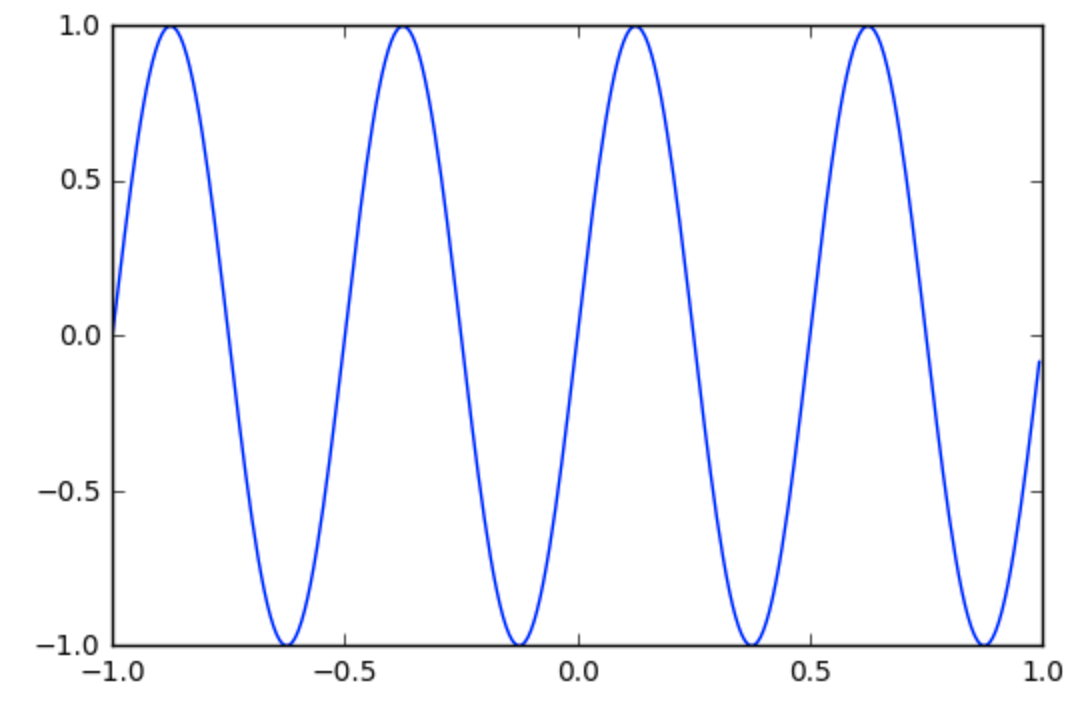
\includegraphics[width=2.7in]{graph1.png}
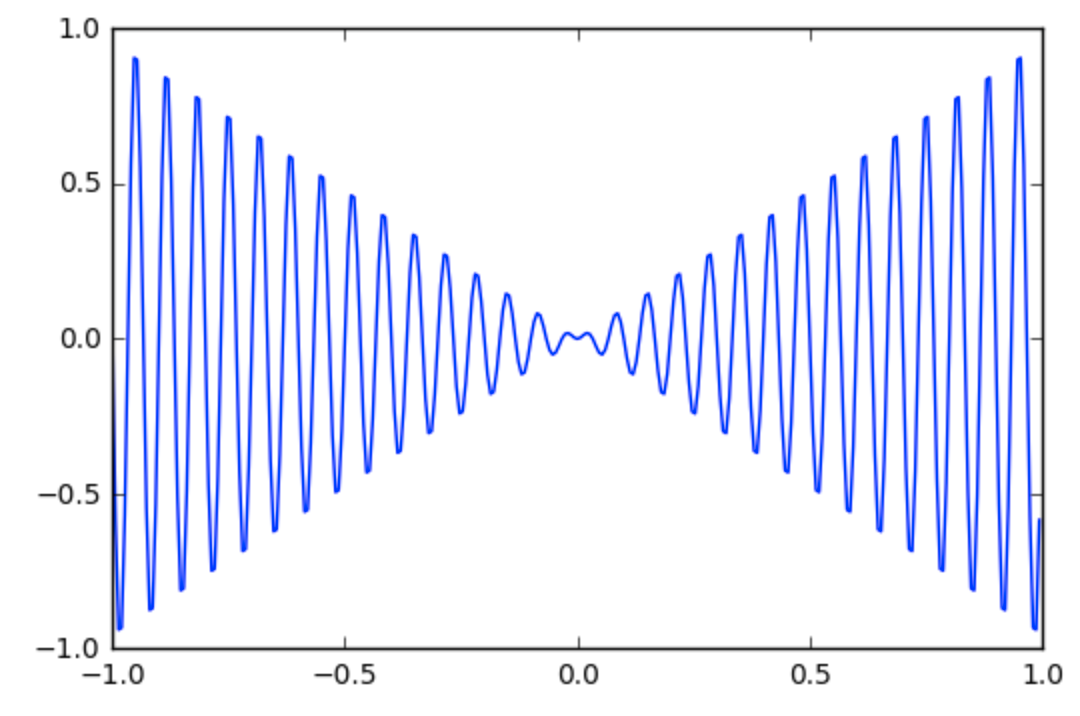
\includegraphics[width=2.7in]{graph2.png}\\
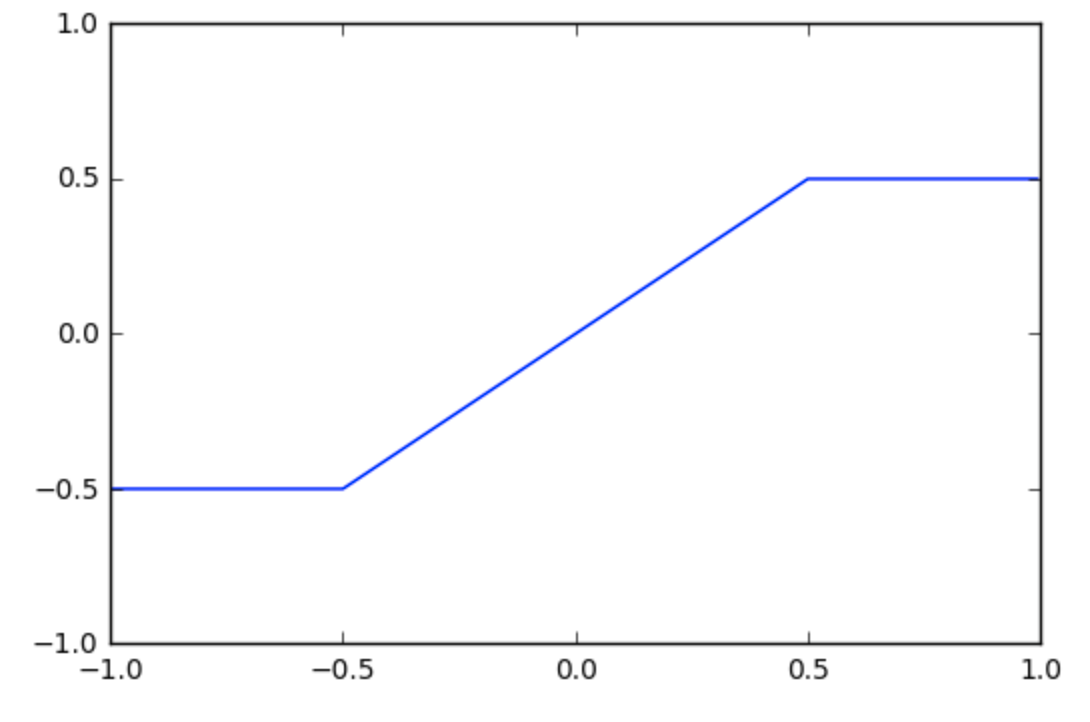
\includegraphics[width=2.7in]{graph3.png}


\subsection*{Problem 2} How do we graph a function $f(x,y)$ in two variables. One way to do it is to consider the function's value $f(x,y)$ at a point $(x,y)$ as the color-intensity at that point. So, for example, if $f(0,0) = 0$, then you put a black pixel at $(0,0)$, i.e. the center. If $f(1,1) = 1$, then you put a white pixel at (1,1), i.e. the top-right. 

Consider the following code and the output:

\begin{lstlisting}
def fun1(x,y):
    return x**2 + y**2
hwlib.drawfunction(fun1) 
\end{lstlisting}

\noindent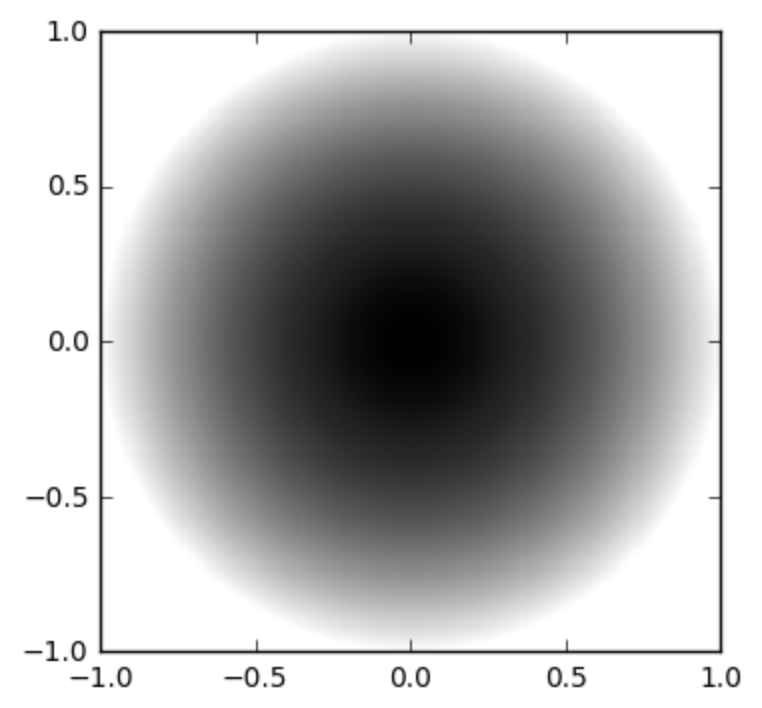
\includegraphics[width=2.7in]{img0.png}

Note that values above $1$ are still represented as white pixels, and values below 0 are represented as black pixels. 

Write down functions that will produce the following pictures:

\noindent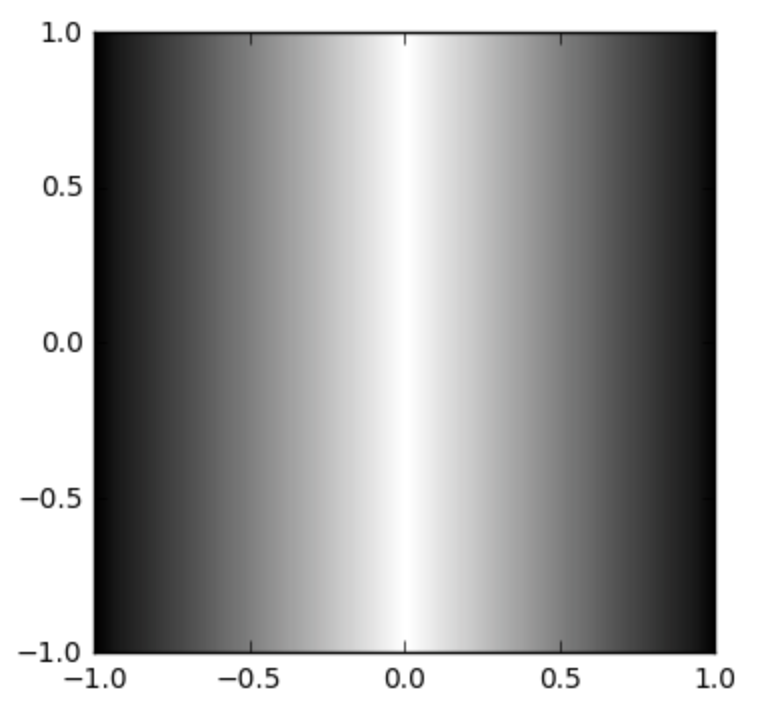
\includegraphics[width=2.7in]{img1.png}
\noindent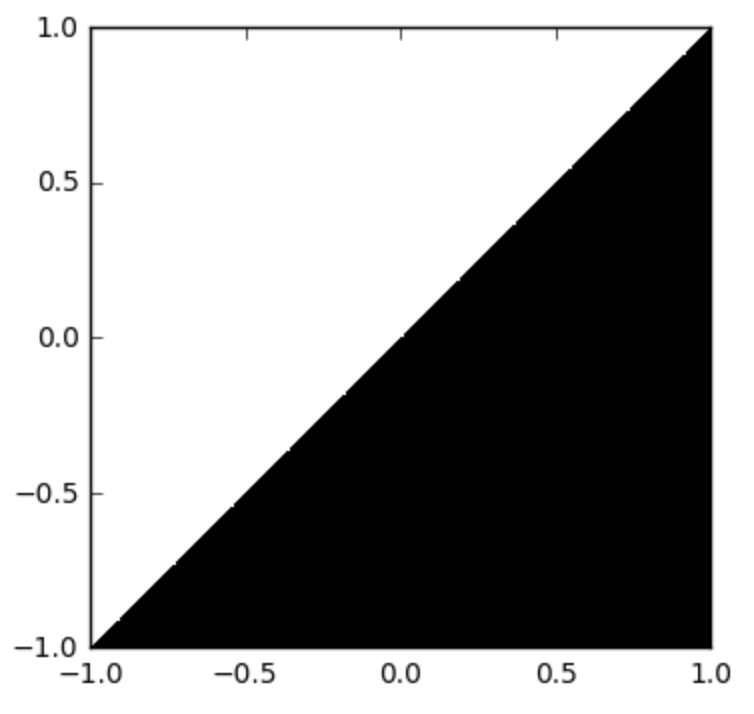
\includegraphics[width=2.7in]{img2.png}\\
\noindent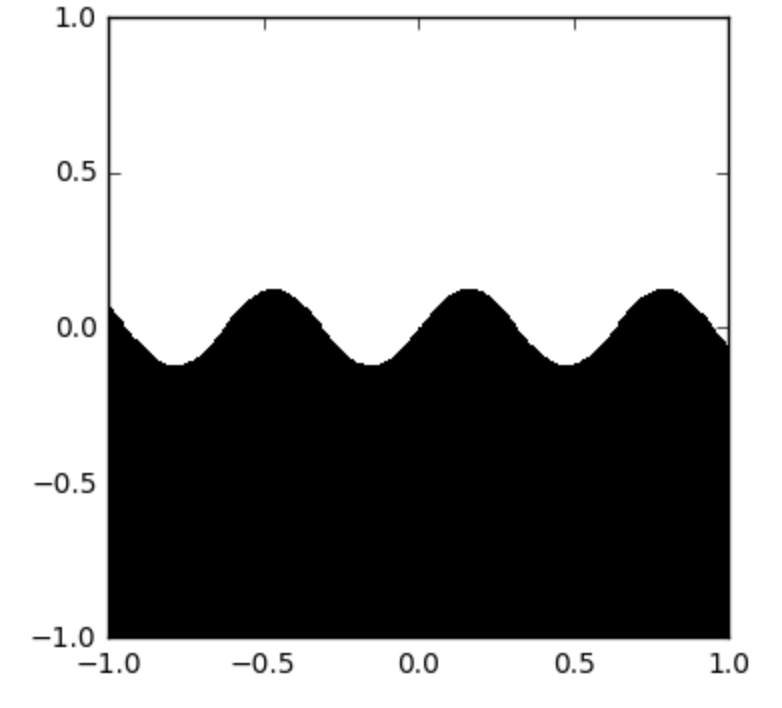
\includegraphics[width=2.7in]{img3.png}
\noindent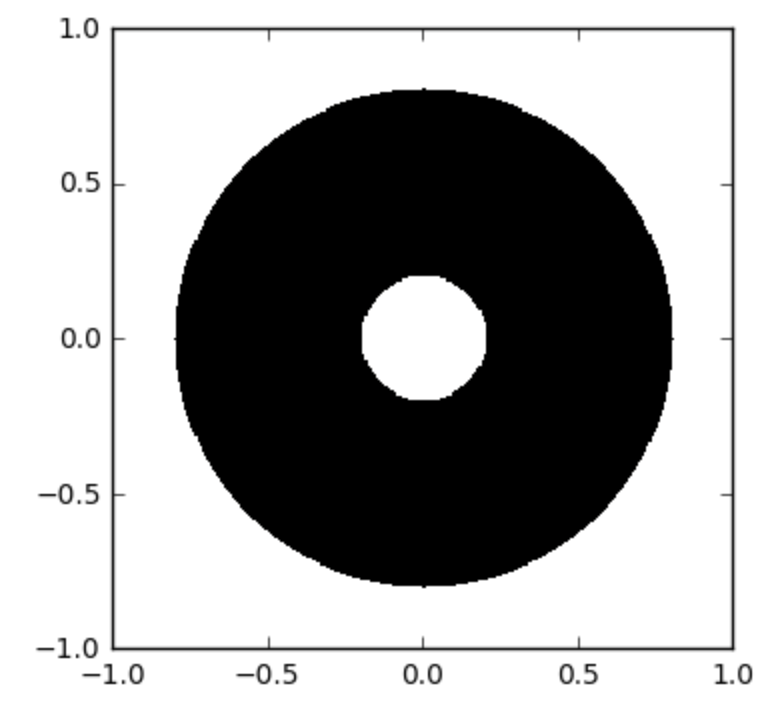
\includegraphics[width=2.7in]{img4.png}\\
\noindent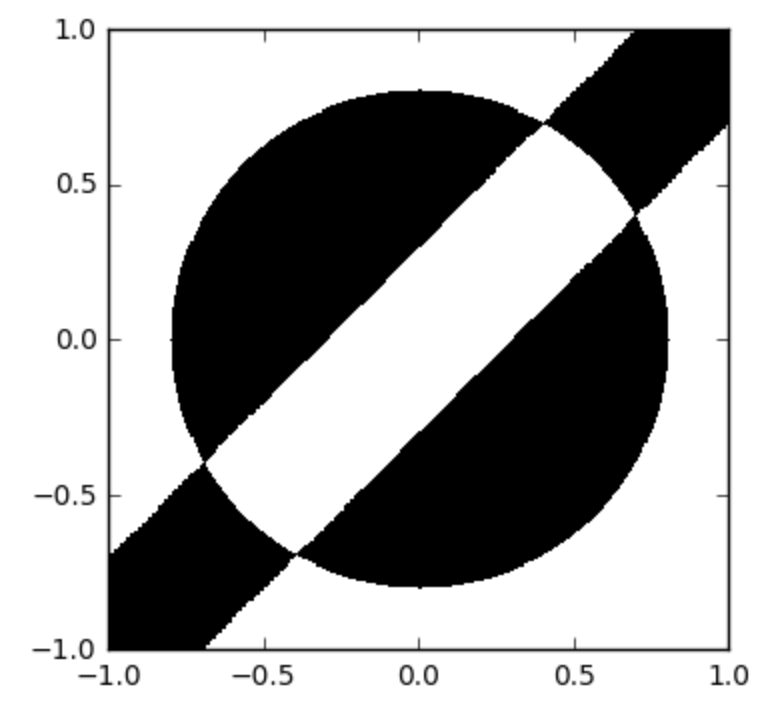
\includegraphics[width=2.7in]{img5.png}
\noindent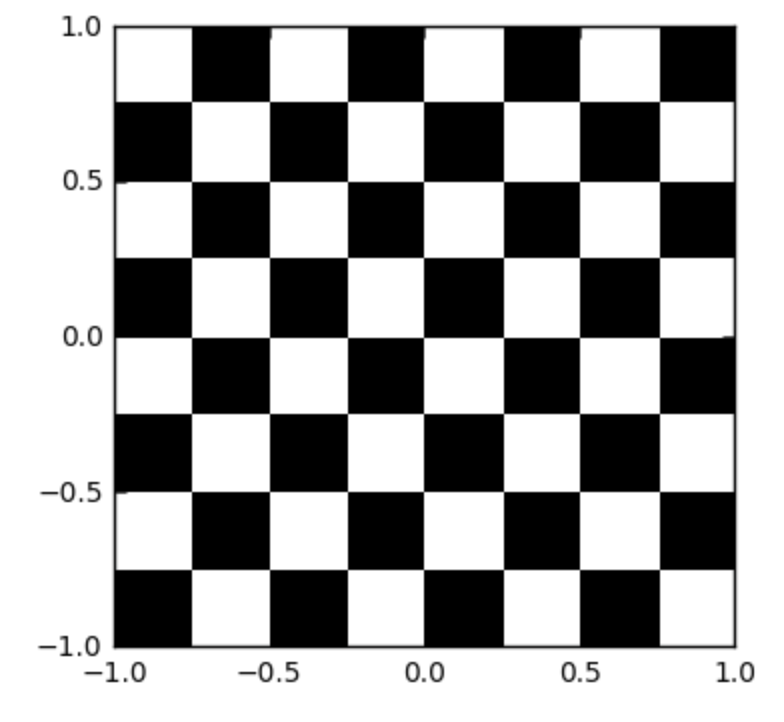
\includegraphics[width=2.7in]{img6.png}

The chessboard is not easy. You may want to use the {\texttt{math.floor}} function. (optional: if you want a bigger challenge, make a function called {\texttt{chessboard(n)}}, which returns a function that, when graphed with drawfunction, will make an $n \times n$ chessboard)

\subsection*{Problem 3} Produce a picture you think is interesting. We will use these to challenge your colleages in the future. 

\subsection*{Problem 4} Functions in python can be used as inputs to a function and can ve returned just like everything else. For example, consider the function {\tt rotateleft} 

\begin{lstlisting}
def rotateleft(f):
    def g(x,y):
        return f(y, -x)
    return g
\end{lstlisting}

It takes in a function and returns a different function which we can then use. For example:

\begin{lstlisting}
def fun(x,y):
    return abs(x+y)
hwlib.drawfunction(fun)
\end{lstlisting}
outputs

\noindent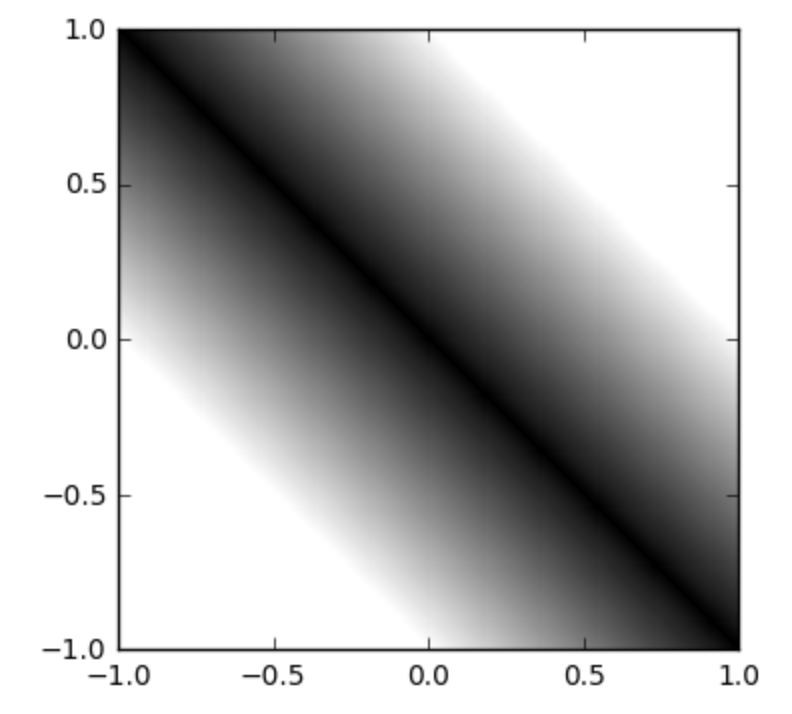
\includegraphics[width=2.7in]{imgorig.png}

What will the following code output? (first guess then try running the code). 

\begin{lstlisting}
hwlib.drawfunction(rotateleft(fun))
\end{lstlisting}

Modify the code for rotateleft so that it rotates to the left by $pi/3$ instead of $pi/2$. 
Then, write a function called repeat. 

\begin{lstlisting}
  def repeat(f):
    def g(x,y):
        ...  
        return ...  
    return g
\end{lstlisting}

such that when we call:

\begin{lstlisting}
hwlib.drawfunction(repeat(fun))
\end{lstlisting}
We get

\noindent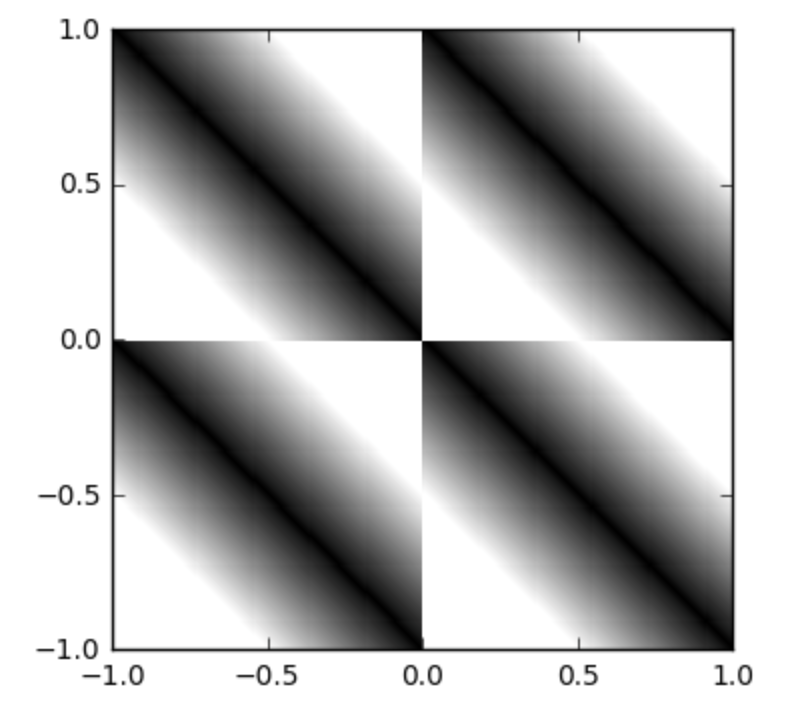
\includegraphics[width=2.7in]{imgrepeat.png}

\end{document}
%%%%%%%%%%%%%%%%%%%%%%%%%%%%%%%%%%%%%%%%%%%%%%%%%%%%%%%%%%%%








